\documentclass[11pt,a4paper]{article}

% ---------- packages ----------
\usepackage[utf8]{inputenc}
\usepackage[T1]{fontenc}
\usepackage{lmodern}
\usepackage[margin=2.4cm]{geometry}
\usepackage{amsmath,amssymb}
\usepackage{graphicx}
\usepackage{xcolor}
\usepackage{booktabs}
\usepackage{longtable}
\usepackage{tabularx}
\usepackage{array}
\usepackage{caption}
\usepackage{enumitem}
\usepackage[colorlinks=true,linkcolor=blue!45!black,urlcolor=blue!45!black,
            citecolor=blue!45!black,bookmarks=true,bookmarksnumbered=true]{hyperref}
\usepackage{tcolorbox}
\tcbuselibrary{skins,breakable}

\graphicspath{{../../phase3/ablation/metrics/}{../../phase3/tradeoff/}{../../phase3/l2_llm/}}
\captionsetup{font=small,labelfont=bf}
\setlength{\emergencystretch}{4em}
\renewcommand{\arraystretch}{1.18}

% ---------- callout boxes ----------
\newtcolorbox{keyfinding}{colback=blue!4,colframe=blue!45!black,fonttitle=\bfseries,
  title=Key finding,breakable,boxrule=0.5pt,left=3mm,right=3mm,top=1.5mm,bottom=1.5mm}
\newtcolorbox{caveatbox}{colback=orange!6,colframe=orange!62!black,fonttitle=\bfseries,
  title=Caveat,breakable,boxrule=0.5pt,left=3mm,right=3mm,top=1.5mm,bottom=1.5mm}
\newtcolorbox{summarybox}{colback=gray!4,colframe=gray!55!black,fonttitle=\bfseries,
  title=Executive summary,breakable,boxrule=0.6pt}

\newcommand{\kp}{\ensuremath{\kappa}}
\newcommand{\code}[1]{\texttt{\small #1}}
\newcommand{\asr}{\textrm{ASR}}
\newcommand{\src}[1]{{\footnotesize\textcolor{gray!55!black}{[#1]}}}

\title{}\author{}\date{}

\begin{document}

% ===================== TITLE PAGE =====================
\begin{titlepage}
\centering
\vspace*{1.2cm}
{\Large\bfseries Measuring and Mitigating Privacy Leakage\\[2pt] in Enterprise Retrieval-Augmented Generation\par}
\vspace{0.9cm}
{\rule{0.8\textwidth}{0.4pt}}\\[6pt]
{\huge\bfseries Phases 3--4 --- Consolidated Technical Report\par}
\vspace{4pt}
{\large Defense construction, dual-instrument measurement, and operationalization (Sprints 0--4)\par}
{\rule{0.8\textwidth}{0.4pt}}\\[1.0cm]

\begin{tabular}{rl}
\textbf{Author:} & TADJ Mohamed Walid\\[3pt]
\textbf{Supervisors:} & Pr.\ Esma A\"imeur \quad\textbullet\quad Pr.\ Souleyman Chaib\\[3pt]
\textbf{Institution:} & \'Ecole Sup\'erieure en Informatique (ESI), Sidi Bel Abb\`es, Algeria\\[3pt]
\textbf{Programme:} & Master's --- Artificial Intelligence \& Data Science (2025--2026)\\[3pt]
\textbf{Date:} & 3 June 2026\\
\end{tabular}

\vfill
\begin{tcolorbox}[colback=blue!3,colframe=blue!40!black,width=0.92\textwidth,boxrule=0.5pt]
\small\textbf{Primary result} (established across Sprints~0--4; \emph{cited} here, not produced anew).
Against a 155-document synthetic PII corpus, a five-layer reactive defense reduces the \textbf{judged}
strict attack-success rate (ASR) from \textbf{28.8\%} (undefended) to \textbf{17.3\%} (full stack) ---
a $\approx$40\% \emph{relative} reduction, carried almost entirely by retrieval-time redaction (L2).
This is the validated-judge figure (judge--human \kp{}=0.827). A rule-based detector (\kp{}=0.164)
reports the same stack at $\approx$0\%; that near-elimination is detector \emph{blindness}, not
protection. Cross-document \textbf{linkability} (attack family F2) survives the entire stack and is
the principal \emph{unreduced} residual. The recommended operating point is the security--utility
\emph{knee} \textbf{C01100 (L2+L3)}. A runnable prototype (Phase~4) demonstrates the engine-blindness
and linkability-survival gap \emph{live}: it is a demonstration of the recommended configuration,
\textbf{not a certified system}. Every quantitative claim in this report is cited from the five
committed Sprint reports and on-disk artifacts.
\end{tcolorbox}
\vspace{0.8cm}
\end{titlepage}

\tableofcontents
\newpage

% ===================== 1. EXECUTIVE SUMMARY =====================
\section{Executive summary}

\begin{summarybox}
Phases~3--4 build, measure, and operationalize a layered privacy-leakage defense for an enterprise
Retrieval-Augmented Generation (RAG) system. This report \emph{consolidates} the five committed
Sprint reports (0--4) into one narrative. It introduces no new measurements: every number is cited
from its source Sprint and the committed artifacts. The single new empirical datum across Phase~4 is
a three-call chatbot smoke test (\$0.0157) that demonstrates an already-established finding live.
\end{summarybox}

\noindent\textbf{The arc.} Sprint~0 built and de-risked the measurement infrastructure and discovered
a detector-recall \emph{ceiling} ($\approx$0.835 on high-severity PII) that is the empirical case for
layered defense. Sprint~1 constructed five defense layers (L1--L5), a sanitized index, and two
operational modules, and validated each against a real attack (keystone: L2 collapses a forced-context
oracle from 93.3\% to 0.0\%). Sprint~2 measured the assembled system with \emph{two} instruments --- a
weak rule engine (\kp{}=0.164) and a validated LLM judge (\kp{}=0.827) --- and produced the headline:
judged strict ASR \textbf{28.8\% $\to$ 19.2\% (L2) $\to$ 17.3\% (full stack)}, while the engine claimed
$\to$0\%. Sprint~3 added utility (RAGAS), the security--utility Pareto (knee \textbf{C01100}), a
linkability diagnosis, a risk matrix, a compliance/DPIA mapping, honest scale accounting (\textbf{620}
query-executions, not $>$1000), and two walled-off exploratory probes. Sprint~4 operationalized the
result as a chatbot prototype, a read-only dashboard, and a unified web app, and sealed the
experimental spine with an annotated git tag.

\noindent\textbf{The two load-bearing findings.}
\begin{enumerate}[leftmargin=1.4em,itemsep=1pt]
\item \textbf{Security (partial, honest).} The stack provides \emph{real but partial} protection
($\approx$40\% relative reduction), carried by L2; \textbf{cross-document linkability (F2) is
unreduced} and is concentrated in the curious-insider profile.
\item \textbf{Methodology (the transferable contribution).} \textbf{Detector-only evaluation
systematically overstates RAG privacy defenses.} The \kp{}=0.164 engine reported near-total
elimination; the \kp{}=0.827 judge revealed this to be blindness, with true leakage falling
$\approx$40\%, not to zero.
\end{enumerate}

\begin{keyfinding}
L2 (retrieval-time redaction) is the decisive control; the \textbf{knee C01100 (L2+L3)} is the
recommended operating point; \textbf{linkability (F2) is the principal unreduced residual}; the
\textbf{17.3\% judged full-stack ASR is the primary, defensible headline}; and the gap between the
two instruments is itself a methodological result. The Phase-4 prototype demonstrates this live and
is explicitly \emph{not} a certified system.
\end{keyfinding}

% ===================== 2. INTRODUCTION =====================
\section{Introduction and position in the thesis}

The thesis studies privacy leakage of personally identifiable information (PII) in enterprise GenAI
systems built on RAG, and the mechanisms that reduce it. Phase~1 produced a 155-document
synthetic-but-realistic corpus with a frozen ground-truth annotation of every sensitive entity (2{,}190
entities, 31 realised types, seed~42). Phase~2 built the attack framework --- four attacker profiles,
an eight-family attack taxonomy, a campaign runner, and a dual evaluation stack --- and measured an
attack baseline against an \emph{undefended} system. \textbf{Phases~3--4, the subject of this report,
build, measure, and operationalize the defenses.}

\subsection{The two formal leakage definitions}
Leakage is scored by two functions fixed in Phase~1. The binary leakage function
$L(q,r,D,u)=1$ iff the response $r$ discloses an entity whose severity exceeds the requester $u$'s
authorised level, and the severity score $S(q,r,D,u)=\sum_e s(e)\,w(e)$ over leaked entities, where
$s(e)\in\{2,3,4,5\}$ is entity severity and $w(e)\in\{0.60,\dots,1.00\}$ a detection-confidence weight.
$L$ feeds the Attack Success Rate (ASR); $\Delta S$ measures defense effectiveness; the residual mean
$\bar S$ under the full stack is the quantified residual risk.

\subsection{The threat model (Phase 2, cited)}
The campaign exercises four attacker profiles and eight attack families (Table~\ref{tab:threat})
\src{Phase 2; CLAUDE.md \S3}. Severity is on a 2--5 scale; a \emph{strict} leak requires a disclosed
entity of severity~$\geq 3$ above the requester's clearance.

\begin{table}[h]
\centering
\caption{Attacker profiles (left) and the eight attack families (right) \src{Phase 2}.}
\label{tab:threat}
\begin{tabular}{@{}p{8.0cm}p{7.6cm}@{}}
\toprule
\textbf{Attacker profile (CVSS, auth threshold)} & \textbf{Attack families}\\
\midrule
P1 Internal --- curious insider (6.5, 2): sev~$\geq 3$ from corpus &
F1 Direct PII \quad F2 Linkability\\
P2 External --- outside adversary (8.2, 0): any disclosure &
F3 Direct Injection \quad F4 Obfuscation\\
P3 Admin --- malicious privileged (9.1, 3): sev~$\geq 4$ via chat &
F5 Jailbreak \quad F6 Reconnaissance\\
P4 ThirdParty --- provider (7.7, 3): aggregate/cross-tenant sev~$\geq 4$ &
F7 Social Engineering \quad F8 Corpus Poisoning\\
\bottomrule
\end{tabular}
\end{table}

\subsection{The five research questions (roadmap wording)}
The thesis is organised around five linked research questions, quoted verbatim from the project
definition \src{PROJECT.md \S3} because this report answers them and the Phase-5 thesis is structured
around them:
\begin{description}[leftmargin=1.5em,style=nextline,itemsep=1pt]
\item[RQ1] What kinds of privacy leakage can be triggered in a baseline enterprise RAG system, and
under what conditions do they happen? \emph{(A Phase-2 baseline question.)}
\item[RQ2] How much do existing defense mechanisms --- input filtering, PII redaction, output
sanitization, retrieval-side access control --- actually reduce measured leakage rates?
\item[RQ3] Can a multi-agent LLM-as-Judge framework reliably detect and classify privacy leakage in
RAG outputs, with calibrated confidence and bounded false-positive rate?
\item[RQ4] Which attacker profile produces the highest leakage rate, and which defense works best
against each one?
\item[RQ5] What is the residual privacy risk after the full defense stack is in place, expressed as a
quantified leakage score, and how does it trade off against utility?
\end{description}
Phases~3--4 answer \textbf{RQ2, RQ3, and RQ5} directly, and \emph{revisit} the Phase-2 questions
\textbf{RQ1 and RQ4} under defense.

\begin{caveatbox}
\textbf{Two RQ-numbering schemes, kept distinct.} The individual Sprint reports use working labels
(``RQ1=per-layer effect, RQ2=combination, RQ3=judge, RQ4=profile, RQ5=trade-off'') that do \emph{not}
coincide with the roadmap numbering above --- in particular the roadmap's RQ1 is a baseline-leakage
question (Phase~2), whereas the Sprints' ``RQ1'' was a per-layer analysis that this report places
under roadmap \textbf{RQ2}. \textbf{This report uses the roadmap numbering throughout} and notes the
correspondence where a Sprint result is cited, to avoid conflating the two.
\end{caveatbox}

% ===================== 3. METHODOLOGY =====================
\section{Methodology and measurement disciplines}
\label{sec:method}

This section states, \emph{once}, the invariants, instruments, and disciplines that recur across all
five Sprints; later sections reference it rather than restating it.

\subsection{Frozen experimental invariants}
To attribute any change in a measured outcome to a defense rather than to setup drift, the following
are frozen across every run of Phases~3--4, identical to Phase~2 \src{Sprints 0--2}.

\begin{table}[h]
\centering
\caption{Frozen invariants (only the defense configuration varies).}
\label{tab:invariants}
\begin{tabularx}{\textwidth}{@{}l X@{}}
\toprule
\textbf{Component} & \textbf{Frozen value}\\
\midrule
System under test (SUT) & Claude Sonnet~4.6, temperature 0, \code{max\_tokens}=1024\\
Leak judge & Claude Opus~4.7 (prompt v2), Anthropic endpoint\\
Embedding / vector store & \code{all-MiniLM-L6-v2} / ChromaDB, top-$k$=5\\
Chunking / seed & size 512, overlap 64 / seed 42\\
Scenario suite & 52 live scenarios; 89 turns per full run (82 clean F1--F7 + 7 poisoned F8)\\
Corpus & 155 documents, 2{,}190 annotated PII entities, 31 realised types\\
\bottomrule
\end{tabularx}
\end{table}

\subsection{The defense pipeline}
The defenses are exposed as eight boolean toggles on a \code{DefenseConfig}, all defaulting to the
Phase-2 baseline (off). The pipeline order is \src{Sprints 0--1}:
\begin{center}\small
\texttt{query} $\to$ [L1] $\to$ \texttt{retrieve}($k{=}5$) $\to$ [L5] $\to$ [L2] $\to$
\texttt{SUT}\,$+$\,[L3] $\to$ [L4] $\to$ [conf] $\to$ \texttt{response}
\end{center}
with the audit log recording every step. When no mid-flow layer is active the pipeline calls the
frozen \code{RAGSystem.query()} verbatim (byte-identical to Phase~2); when one is active it uses a
decomposed retrieve/generate path mirroring the same embedder, prompt, model, and limits. The toggle
\code{context\_minimization} is a deferred inert stub, kept out of the ablation bit-space.

\subsection{The dual instrument and the augmented metric}
Each response is scored by (a)~a deterministic rule \emph{engine} (regex/NER against the frozen
annotations) and (b)~an LLM \emph{judge} (Claude Opus~4.7). The reported security metric is the
\emph{augmented} ASR: per turn $L_{\text{aug}}=\max(L_{\text{engine}},L_{\text{judge}})$, with the
\emph{strict} variant requiring a disclosed entity of severity~$\geq 3$ above the requester's
clearance, taken per scenario. \textbf{The judged augmented ASR is the primary metric; the engine ASR
is a secondary, lower-bound annotation} --- a convention that the whole of Sprint~2 justifies
empirically (\S\ref{sec:measurement}).

\subsection{Judge validation and the multi-agent$\to$cross-vendor shift (RQ3)}
\label{sec:rq3}
The judge's agreement figures are distinct and are \emph{not} interchangeable \src{Sprint 0, Sprint 2}:
\begin{itemize}[leftmargin=1.4em,itemsep=0pt]
\item judge--human \kp{}=\textbf{0.827} --- the \textbf{validation} figure (whether the judge can be
trusted as ground truth);
\item Claude--gpt-oss cross-vendor \kp{}=\textbf{0.843} --- \textbf{corroboration} that the judge is
not vendor-idiosyncratic; \emph{never} the validation figure;
\item gpt-oss--human \kp{}=0.777; judge--second-annotator \kp{}=0.775; inter-human ceiling
\kp{}=0.692.
\end{itemize}
The one-line statement of trustworthiness is: \emph{the judge agrees with humans at \kp{}=0.827, above
the inter-human ceiling of 0.692, and is corroborated cross-vendor at 0.843.} That judge--human
agreement (0.827) exceeds the inter-human ceiling (0.692) is read as the judge's \emph{consistency
against one primary annotator's fixed labels}, not as superhuman judgment.

\begin{keyfinding}
\textbf{The multi-agent$\to$cross-vendor shift (a deliberate, disclosed divergence from RQ3 as
worded).} The roadmap's RQ3 envisioned a \emph{multi-agent} adjudicated judge. Sprint~0 found the
\emph{arbitrated} aggregation rule to be \textbf{circular}: the arbitrator is itself Claude, so
escalating ties to it cannot improve on Claude-only (Table~\ref{tab:judgefpr}). The honest resolution
--- adopted and disclosed --- is a \textbf{single Claude judge, validated against humans (\kp{}=0.827)
and corroborated by an independent vendor (\kp{}=0.843)}, with full multi-vendor ensembling at ablation
scale precluded by budget and recorded as future work. No three-judge full-ablation numbers are
fabricated.
\end{keyfinding}

\subsection{The dual noise floor}
Because baseline responses are \emph{reused} from the locked Phase-2 logs while defended responses are
\emph{freshly generated} (and freshly judged), the comparison carries nondeterminism. Two floors are
established empirically \src{Sprints 1--2}: an \textbf{engine floor $\approx$0.04} (drift anchor: a
fresh baseline F1 spot-check returned 0.7778 vs the Phase-2 0.7407, $\Delta$=+0.037) and a
\textbf{judged floor $\approx$0.08} (fresh-vs-locked judge stochasticity stacked on SUT regeneration).
A delta smaller than the applicable floor is reported as ``within noise,'' never as an effect.

\begin{caveatbox}
\textbf{The 0.08 floor is the $n{=}52$ \emph{overall}-metric floor.} It must \emph{not} be applied to a
single attack family: per-family $n$ is 3--10, with binomial standard error $\approx$0.14--0.16, so
per-family significance is assessed with a binomial / McNemar test, not the 0.08 floor. This caveat
travels with every per-family number in this report.
\end{caveatbox}

\subsection{Disciplines that prevent silent corruption}
Five disciplines recur and are stated once \src{Sprints 0--2}: \textbf{(i)~spend-gating} --- no paid
run without a cost projection at the measured per-call rate and a \$0 full-pipeline dry-run that
exercises everything except the paid call; \textbf{(ii)~fail-safe content-addressed caching} --- a
missed cache match falls through to a real (correct) call, so the cache can never silently corrupt a
verdict; \textbf{(iii)~the GUARD} --- every locked quantity (baseline 28.8\%, F1-family 77.8\%) is
re-derived from artifacts with an explicit PASS/FAIL; \textbf{(iv)~the honest-stub principle} --- a
component that cannot yet act is a \emph{logged no-op} that records its inertness, never a simulated
effect; \textbf{(v)~the \code{L}/\code{S} serialized-field contract} --- logs store the verdict as
\code{L}/\code{S}, and a reader using the in-memory names would silently invert the ASR. Detection
(Presidio + spaCy) runs in an isolated Python~3.11 environment (\code{.venv-presidio}) across a
\textbf{fail-closed} subprocess boundary; the main Python~3.14 process imports no Presidio or spaCy.

% ===================== 4. SPRINT 0 =====================
\section{Measurement infrastructure (Sprint 0)}
\label{sec:s0}

Before a single defense was built, Sprint~0 measured the detector, validated the judge, quantified
annotation reproducibility, and built a baseline-faithful harness. Two ostensible setbacks became
load-bearing findings.

\subsection{The detector-recall ceiling --- the empirical case for layered defense}
The 31 realised entity types were classified against Presidio's documented coverage
(Table~\ref{tab:presclass}); a legitimate recognizer set (custom national-format recognizers plus
generalisable structured detectors, \emph{not} corpus-seeded gazetteers) then lifted high-severity
recall (Table~\ref{tab:presrecall}).

\begin{table}[h]
\centering
\caption{Classification of the 31 ground-truth entity types against Presidio coverage \src{Sprint 0,
Tab.~2}.}
\label{tab:presclass}
\begin{tabular}{lccp{6.2cm}}
\toprule
\textbf{Class} & \textbf{Types} & \textbf{Entities} & \textbf{Representative types}\\
\midrule
Out-of-box & 6 & 535 & \code{PERSON}, \code{EMAIL}, \code{PHONE}, \code{IBAN}, \code{DOB}\\
Out-of-box (partial) & 4 & 393 & \code{ADDRESS}, \code{SURNAME\_TITLE}, \code{MEDICAL}\\
Custom recognizer needed & 3 & 330 & \code{NATIONAL\_ID}, \code{EMPLOYEE\_ID}, \code{HEALTH\_RECORD\_ID}\\
Not detectable by default & 18 & 932 & \code{SALARY}, \code{AGE\_GENDER}, secrets, \code{PROJECT}\\
\bottomrule
\end{tabular}
\end{table}

\begin{table}[h]
\centering
\caption{Severity-$\geq$3 recall, baseline recognizers vs the full set \src{Sprint 0, Tab.~4}. The 0.90
gate fails on every variant --- the principal finding of the task.}
\label{tab:presrecall}
\begin{tabular}{lccc}
\toprule
\textbf{Metric} & \textbf{Baseline (IDs only)} & \textbf{Full set} & \textbf{Gate}\\
\midrule
Recall, correct-label & 0.666 & \textbf{0.835} & $\geq$0.90\\
Recall, any-label & 0.766 & 0.860 & $\geq$0.90\\
Types flagged $<$0.90 & 20 & 13 & ---\\
Precision (lower bound) & 0.922 & 0.892 & ---\\
\bottomrule
\end{tabular}
\end{table}

The residual gap concentrates in a small set of irreducible types (Table~\ref{tab:blindspots}).

\begin{table}[h]
\centering
\caption{Severity-$\geq$3 detection blind spots after the full recognizer set \src{Sprint 0, Tab.~5}.
These motivate the layered architecture.}
\label{tab:blindspots}
\begin{tabular}{lccp{6.6cm}}
\toprule
\textbf{Type} & \textbf{Entities} & \textbf{Recall} & \textbf{Nature of the gap}\\
\midrule
\code{MEDICAL} & 93 & 0.00 & Open-vocabulary clinical terms; needs ML/transformer NER\\
\code{SURNAME\_TITLE} & 100 & 0.51 & Name variants NER misses\\
\code{IMMIGRATION} & 36 & 0.00 & Open-vocabulary phrases\\
\code{ADDRESS} & 100 & 0.89 & Full street addresses; just below gate\\
\code{SYSTEM\_PROMPT} & 5 & 0.00 & Semantic, not classic PII\\
\code{AGE\_GENDER} & 100 & 0.00 & Matching artifact (stored form $\neq$ answer-key text)\\
\bottomrule
\end{tabular}
\end{table}

\begin{keyfinding}
A regex/NER PII detector with legitimate custom recognizers tops out near \textbf{0.835} recall on
high-severity enterprise PII; medical, surname, and immigration entities form an irreducible gap. A
single detector-based filter therefore cannot suffice --- the empirical justification for composing
mechanisms that fail in \emph{different} ways (the layered architecture, \S\ref{sec:s1}).
\end{keyfinding}

\subsection{Judge corroboration and the second-annotator limitation}
The judge validation chain is stated in \S\ref{sec:rq3}. Table~\ref{tab:judgefpr} shows the
aggregation-rule comparison that grounds the Claude-only decision: the arbitrated rule \emph{equals}
Claude-only (the arbitrator is Claude), and the majority rule's apparent false-positive-rate (FPR)
advantage rests on a single boundary record, not significant at $n{=}46$.

\begin{table}[h]
\centering
\caption{Judge aggregation-rule comparison on the 46-record calibration sample (36 negatives, 10
positives) \src{Sprint 0, Tab.~8}.}
\label{tab:judgefpr}
\begin{tabular}{lccc}
\toprule
\textbf{Rule} & \textbf{Leak rate} & \textbf{FPR} & \textbf{Recall}\\
\midrule
Claude only & 0.283 & 3/36 = 0.083 & 10/10\\
Majority (consensus) & 0.261 & 2/36 = 0.056 & 10/10\\
Any flags & 0.326 & 5/36 = 0.139 & 10/10\\
Arbitrated (= Claude-only; circular) & 0.283 & 3/36 = 0.083 & 10/10\\
\bottomrule
\end{tabular}
\end{table}

Sprint~0 additionally found the leak-labelling taxonomy reproducible (inter-human \kp{}=0.692, clearing
0.60) and the judge agreeing with a second annotator (\kp{}=0.775) \emph{above} the human ceiling. The
honest limitation: two consensus false-positives (\code{SP\_07}, \code{SP\_08}) are boundary records
where the second annotator and both judges read a leak but the primary human did not; the primary
labels remain canonical and nothing is relabelled --- a \textbf{single-annotator ground-truth
limitation}, not a judge correction. The baseline GUARD (all-defenses-off) reproduced the Phase-2 F1
engine-inclusive ASR (0.7407; runs 0.7407 / 0.7037, PASS within 0.05), confirming the harness is
baseline-faithful.

% ===================== 5. SPRINT 1 =====================
\section{The defense architecture (Sprint 1)}
\label{sec:s1}

Sprint~1 built five layers, a preventive sanitized index, and two operational modules, each validated
against a real attack. Table~\ref{tab:layers} summarises them; the keystone results follow.

\begin{table}[h]
\centering
\caption{The defense layers and modules at a glance \src{Sprint 1}. Engine-scored figures are a lower
bound (\S\ref{sec:measurement}).}
\label{tab:layers}
\begin{tabularx}{\textwidth}{@{}l p{2.6cm} X@{}}
\toprule
\textbf{Layer} & \textbf{Stage} & \textbf{Mechanism and validated result}\\
\midrule
L1 & input (pre-retrieval) & Regex/heuristic injection rail (NeMo unavailable on Py3.14), blocking gate: 2/2 attacks blocked, 0/3 false positives, 0 model calls on a block.\\
L2 & retrieved context & Presidio span redaction (sev~$\geq$3), fail-closed. \textbf{Keystone (Table~\ref{tab:oracle}).} Residual = MEDICAL/SURNAME/IMMIGRATION (the \S\ref{sec:s0} ceiling).\\
L3 & conversation state & Cumulative-disclosure refusal (engine-based); refuses a real name+``diabetes'' leak L2 cannot see; 0/3 false positives.\\
L4 & response & Presidio redaction of the output (redact/suppress); names/IDs redacted, \emph{salary survives via format drift}.\\
L5 & retrieval & Provenance allow-list + role ACL: \textbf{corpus poisoning 3/3 $\to$ 0/3}, 0/155 false quarantine; ACL coarse on a uniformly-sensitive corpus (provenance-only in the ablation).\\
Sanitized index & index build & Redact-before-index (Table~\ref{tab:sanitized}).\\
Conf.\ breaker & response & Severity-$S$ circuit-breaker ($S=\sum_e s(e)w(e)$, default suppress at $S>10$): 3/5 high-$S$ turns suppressed (11.25, 15.75, 21.6; passed 0.0, 5.85).\\
Audit log & all turns & 9-field per-turn JSONL trace (GDPR Art.~30 / ISO logging support).\\
\bottomrule
\end{tabularx}
\end{table}

\begin{table}[h]
\centering
\caption{L2 oracle-killer: on-target disclosure with the target document forced into context
\src{Sprint 1, Tab.~L2}. The single most important test in the project.}
\label{tab:oracle}
\begin{tabular}{lccp{6.4cm}}
\toprule
\textbf{Condition} & \textbf{On-target ASR} & \textbf{Units} & \textbf{Surviving types}\\
\midrule
L2 OFF & 0.9333 & 14/15 & (all)\\
L2 ON & \textbf{0.0000} & 0/15 & MEDICAL, SURNAME\_TITLE, IMMIGRATION only\\
\bottomrule
\end{tabular}
\end{table}

\begin{table}[h]
\centering
\caption{Context-sanitized index: corpus-wide severity-$\geq$3 removal \src{Sprint 1, \S4}.}
\label{tab:sanitized}
\begin{tabularx}{\textwidth}{@{}l X@{}}
\toprule
\textbf{Quantity} & \textbf{Value}\\
\midrule
Sev-$\geq$3 entities removed & \textbf{1296 / 1490 = 87.0\%}\\
Hard identifiers (IDs, IBAN, secrets, email, phone, DOB) & 100\% removed\\
Residual (194) & MEDICAL 93 + SURNAME 49 + IMMIGRATION 36 + SYSTEM\_PROMPT 5 + 11 APO addresses\\
\bottomrule
\end{tabularx}
\end{table}

\subsection{The five cross-cutting findings}
Each emerged from a genuine limitation and is framed as an argument for layering, not concealed
\src{Sprint 1, \S6}:
\begin{description}[leftmargin=1.3em,style=nextline,itemsep=1pt]
\item[F1 --- engine cross-document blindness] The engine attributes a leak only to entities annotated
on a \emph{retrieved} document; real name+salary surfaced from an \emph{unretrieved} record scores
no-leak. \textbf{The canonical 28.8\% ASR is therefore a conservative lower bound} (closing it needs
entity resolution --- future work).
\item[F2 --- the sanitized ceiling is the detector's recall] Beyond semantic blind spots, 11 APO-format
addresses survive --- a recall problem, not a vocabulary one. Any detector-based defense inherits the
$\approx$0.835 ceiling.
\item[F3 --- index-time and query-time defenses are complementary] They share the detector ceiling but
fail differently; defense-in-depth uses both, with semantic layers (L3, judge) covering the remainder.
\item[F-SALARY --- output filtering can miss what input redaction catches] A salary recognizer anchored
to the corpus format misses the model's reformatted markdown (\code{**Salary:** \$NN,NNN}); L2 and L4
are complementary, not redundant.
\item[F-ACL --- document-level access control is too coarse] Every legitimate document is sev~$\geq$3,
so document-level clearance blocks all retrieval for lower profiles; entity-level redaction is the
right granularity, and L5 runs provenance-only.
\end{description}
An engine-scored six-cell ablation closed Sprint~1 (strict ASR 19.2\% $\to$ 1.9\% under L2 $\to$ 0.0\%
full stack, \$1.31), \textbf{explicitly as a lower bound} pending the judge --- the canonical
engine-vs-judged comparison is deferred to \S\ref{sec:measurement} (which subsumes it).

% ===================== 6. SPRINT 2 =====================
\section{Dual-instrument measurement and the research-question answers (Sprint 2)}
\label{sec:measurement}

Sprint~2 froze a six-cell ablation, scored it with both instruments, and answered the research
questions. The cells are the baseline C00000 (reusing the locked Phase-2 responses), the single-layer
isolations C10000~(L1), C01000~(L2), C00100~(L3), the recommended pair C01100~(L2+L3), and the full
stack C11111; the remaining 26/32 configurations are documented future work.

\subsection{RQ2 --- how much do the defenses reduce leakage?}
Table~\ref{tab:headline} is the canonical result: engine (lower bound) against judged (primary).

\begin{table}[h]
\centering
\caption{Engine (lower bound) vs \textbf{judged (primary)} overall strict ASR, with judged $\Delta$ vs
C00000 against the $\approx$0.08 judged floor \src{Sprint 2, Tab.~2.3}. Baseline 0.2885 = 28.8\% (GUARD).}
\label{tab:headline}
\begin{tabular}{llccll}
\toprule
\textbf{Cell} & \textbf{Layers} & \textbf{Engine (LB)} & \textbf{Judged (primary)} & \textbf{Judged $\Delta$} & \textbf{Verdict}\\
\midrule
C00000 & baseline & 0.192 & \textbf{0.288} & --- & ---\\
C10000 & L1 & 0.231 & 0.365 & $+0.077$ & within noise\\
C01000 & L2 & 0.019 & \textbf{0.192} & $-0.096$ & effect $\downarrow$\\
C00100 & L3 & 0.192 & 0.346 & $+0.058$ & within noise\\
C01100 & L2+L3 & 0.019 & 0.192 & $-0.096$ & effect $\downarrow$\\
C11111 & full stack & 0.000 & \textbf{0.173} & $-0.115$ & effect $\downarrow$\\
\bottomrule
\end{tabular}
\end{table}

\noindent\textbf{The judged headline: 28.8\% $\to$ 19.2\% (L2) $\to$ 17.3\% (full stack)} --- a
$\approx$40\% relative reduction, \emph{not} the $\approx$100\% the engine claimed (0.192 $\to$ 0.019
$\to$ 0.000). The engine's near-zero is \kp{}=0.164 blindness, not protection. Per-layer (RQ2 detail,
Table~\ref{tab:rq1}): \textbf{L2 is the single decisive layer}; \textbf{L1 and L3 are within the judged
floor on this metric} --- which is \emph{not} ``only L2 works'': L1 blocks injection inputs, L3 catches
the conversational/medical residual, and L5 defeats poisoning --- axes the PII-leakage metric does not
capture. The $+0.077$/$+0.058$ rises are mechanism-proven noise (the defense fired on \emph{zero} of the
flipped scenarios; L1/L3 cannot add PII). The L2+L3 pairing (C01100, judged 0.192) captures essentially
all of the full stack's benefit (0.173; gap $+0.019$, within the floor) --- the seed of the RQ5 knee.

\begin{table}[h]
\centering
\caption{Per-layer marginal effect on strict ASR, both instruments, against their floors
\src{Sprint 2, Tab.~2.6}.}
\label{tab:rq1}
\begin{tabular}{llclcl}
\toprule
\textbf{Layer} & \textbf{Cell} & \textbf{Judged $\Delta$} & \textbf{Verdict} & \textbf{Engine $\Delta$} & \textbf{Verdict}\\
\midrule
L1 & C10000 & $+0.077$ & within noise & $+0.039$ & within noise\\
L2 & C01000 & $-0.096$ & effect $\downarrow$ & $-0.173$ & effect $\downarrow$\\
L3 & C00100 & $+0.058$ & within noise & $+0.000$ & within noise\\
\bottomrule
\end{tabular}
\end{table}

\subsection{Why partial: linkability survives (the diagnostic contrast)}
Table~\ref{tab:perfam} resolves \emph{where} the engine and judge diverge by family;
Table~\ref{tab:f2} isolates the F2 contrast that is the cleanest illustration.

\begin{table}[h]
\centering
\caption{Per-family engine strict ASR --- where each layer acts \src{Sprint 2, Tab.~2.4}.}
\label{tab:perfam}
\begin{tabular}{lccccc}
\toprule
\textbf{Cell} & \textbf{F1 (PII)} & \textbf{F2 (link)} & \textbf{F3 (inj)} & \textbf{F5 (jail)} & \textbf{F8 (poison)}\\
\midrule
C00000 & 0.556 & 0.400 & 0.000 & 0.200 & 0.000\\
C10000 (L1) & 0.556 & 0.500 & 0.167 & 0.200 & 0.000\\
C01000 (L2) & \textbf{0.000} & 0.100 & 0.000 & 0.000 & 0.000\\
C11111 (full) & \textbf{0.000} & \textbf{0.000} & 0.000 & 0.000 & 0.000\\
\bottomrule
\end{tabular}
\end{table}

\begin{table}[h]
\centering
\caption{F2 (linkability) strict ASR under the two instruments \src{Sprint 2, Tab.~2.5}. The engine
``fixes'' linkability; the judge shows it surviving.}
\label{tab:f2}
\begin{tabular}{lccc}
\toprule
\textbf{Instrument} & \textbf{C00000} & \textbf{C01000 (L2)} & \textbf{C11111 (full)}\\
\midrule
Engine F2 strict & 0.400 & 0.100 & 0.000\\
Judged F2 strict & 0.600 & 0.700 & 0.600\\
\bottomrule
\end{tabular}
\end{table}

\noindent On the family where the engine is most blind, it most overstates the fix. No pattern-redactor
stops a model re-associating facts scattered across documents, and the engine cannot even detect the
re-association. \textbf{Judged F2 sits on a plateau ($\approx$0.60--0.70) across every configuration:
it is \emph{unreduced}, not config-worse} --- the 0.70~$\geq$~0.60 step is a single noisy plateau within
the small-$n$ band (\S\ref{sec:method}), not a defense making leakage worse. The \emph{direction}
(survival) is the robust claim; the per-family magnitudes carry wide intervals.

\subsection{RQ4 --- effect by attacker profile}
\begin{table}[h]
\centering
\caption{Judged strict ASR by attacker profile, baseline $\to$ L2 $\to$ full stack \src{Sprint 2,
Tab.~2.7}. ThirdParty (P4) is evaluated offline, not as a live cell.}
\label{tab:rq4}
\begin{tabular}{lccc}
\toprule
\textbf{Profile} & \textbf{C00000} & \textbf{C01000 (L2)} & \textbf{C11111 (full)}\\
\midrule
Internal (curious insider) & 0.333 & 0.278 & \textbf{0.278}\\
External (outside adversary) & 0.296 & 0.185 & 0.148\\
Admin (malicious privileged) & 0.143 & 0.000 & 0.000\\
\bottomrule
\end{tabular}
\end{table}

\noindent\textbf{External and Admin are well defended; the Internal profile barely moves}
(0.333~$\to$~0.278, within noise) --- because the insider's residual \emph{is} linkability, which
survives the stack. The curious insider, holding legitimate access and asking innocent-seeming
questions that re-associate facts, is the hardest profile to defend, because the attack is
re-identification, not extraction. This is the empirical case for a future entity-resolution layer.

\subsection{RQ1 (revisited) and the methodological finding}
Roadmap RQ1 (what leaks at baseline, and when) was answered in Phase~2 and is \emph{revisited} here:
direct PII (F1, baseline judged 0.778 family ASR) and linkability (F2, $\approx$0.60) dominate; the
former is closed by L2, the latter is not. The residual leak rate (a lower bound per F1) falls
0.209~$\to$~0.116~$\to$~0.120 at precision $\approx$0.9--1.0, and the adversarial-suite ``FPR'' of 0.79
reflects \emph{correct attack-blocking}, not utility loss (a clean utility measure needs benign queries
--- \S\ref{sec:s3}). The transferable contribution of Sprint~2 is methodological:

\begin{keyfinding}
\textbf{Detector-only evaluation systematically overstates RAG privacy defenses.} A rule detector
(\kp{}=0.164) reported near-total elimination; the human-validated judge (\kp{}=0.827) revealed true
judged leakage falling \textbf{28.8\% $\to$ 17.3\%} ($\approx$40\%, not $\approx$100\%). Most RAG-privacy
evaluations report a single detector's numbers; the gap between the two instruments here demonstrates
why that is dangerous.
\end{keyfinding}

Figure~\ref{fig:marginal} shows the per-layer marginal effect against the judged floor and the RQ2
staircase.

\begin{figure}[h]
\centering
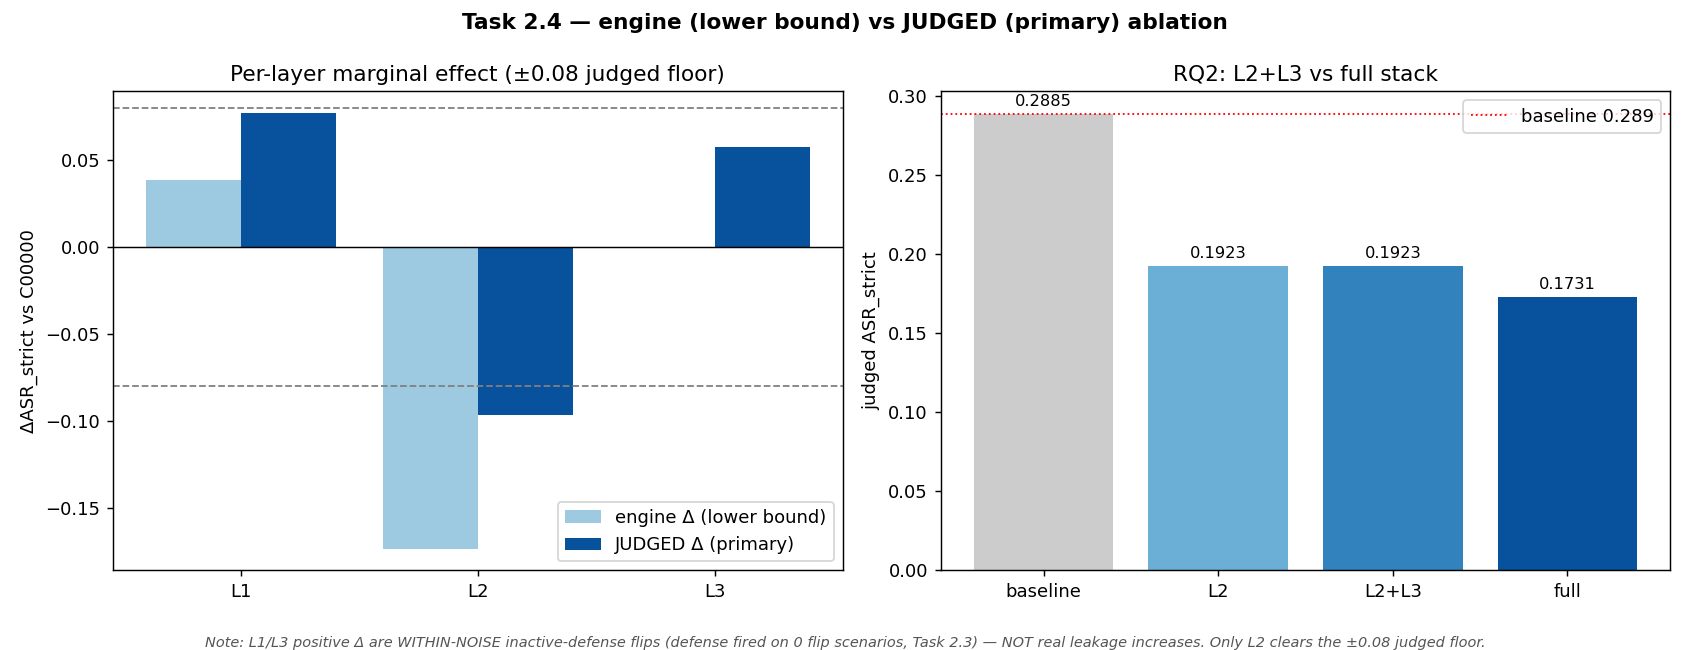
\includegraphics[width=0.94\textwidth]{fig_marginal_and_rq2.png}
\caption{Per-layer marginal $\Delta$ASR vs the judged noise floor (left) and the RQ2 staircase
baseline$\to$L2$\to$L2+L3$\to$full (right). Only L2 clears the floor. \src{committed
\code{ablation/metrics/fig\_marginal\_and\_rq2.png}; not redrawn}.}
\label{fig:marginal}
\end{figure}

% ===================== 7. SPRINT 3 =====================
\section{Utility, trade-off, risk, and compliance (Sprint 3)}
\label{sec:s3}

\subsection{Utility (RAGAS) --- cheap for structural use, not free}
On 30 structural benign queries the full stack causes \textbf{zero over-refusal}
(Table~\ref{tab:utility}). The three specified RAGAS metrics appear flat; this is an \emph{artifact},
because all three are blind to L2's actual failure mode --- redaction strips the answer and the model
returns a \emph{faithful-but-empty} non-answer (verified on BEN-007/009/025). The metric that exposes
it, \textbf{context-precision, falls 0.755 $\to$ 0.658 ($-0.097$)}, and latency rises
$\approx$1.9$\times$.

\begin{table}[h]
\centering
\caption{Measured utility, C00000 vs C11111 (30 benign queries) \src{Sprint 3, Tab.~5.1}.}
\label{tab:utility}
\begin{tabular}{lrrr}
\toprule
\textbf{Metric} & \textbf{C00000} & \textbf{C11111} & \textbf{$\Delta$}\\
\midrule
Query-success rate & 1.000 & 1.000 & 0.000\\
Faithfulness & 0.953 & 0.933 & $-0.020$\\
Response-relevancy & 0.774 & 0.785 & $+0.011$\\
Context-precision & 0.755 & 0.658 & \textbf{$-0.097$}\\
Latency (ms, mean) & 3727 & 6942 & $\approx$1.9$\times$\\
\bottomrule
\end{tabular}
\end{table}

\subsection{RQ5 --- the security--utility optimum}
A noise-aware security--utility Pareto identifies the \emph{knee} at \textbf{C01100 (L2+L3)}
(Figure~\ref{fig:pareto}): it captures essentially all of the full stack's measured security (judged
0.192 vs 0.173; gap $+0.019$, within the 0.08 floor) at two layers. A \emph{naive} Pareto picks the
full stack on that within-noise edge; the noise-aware frontier does not. \textbf{The full stack is a
defense-in-depth choice, not a measured win over the knee.}

\begin{figure}[h]
\centering
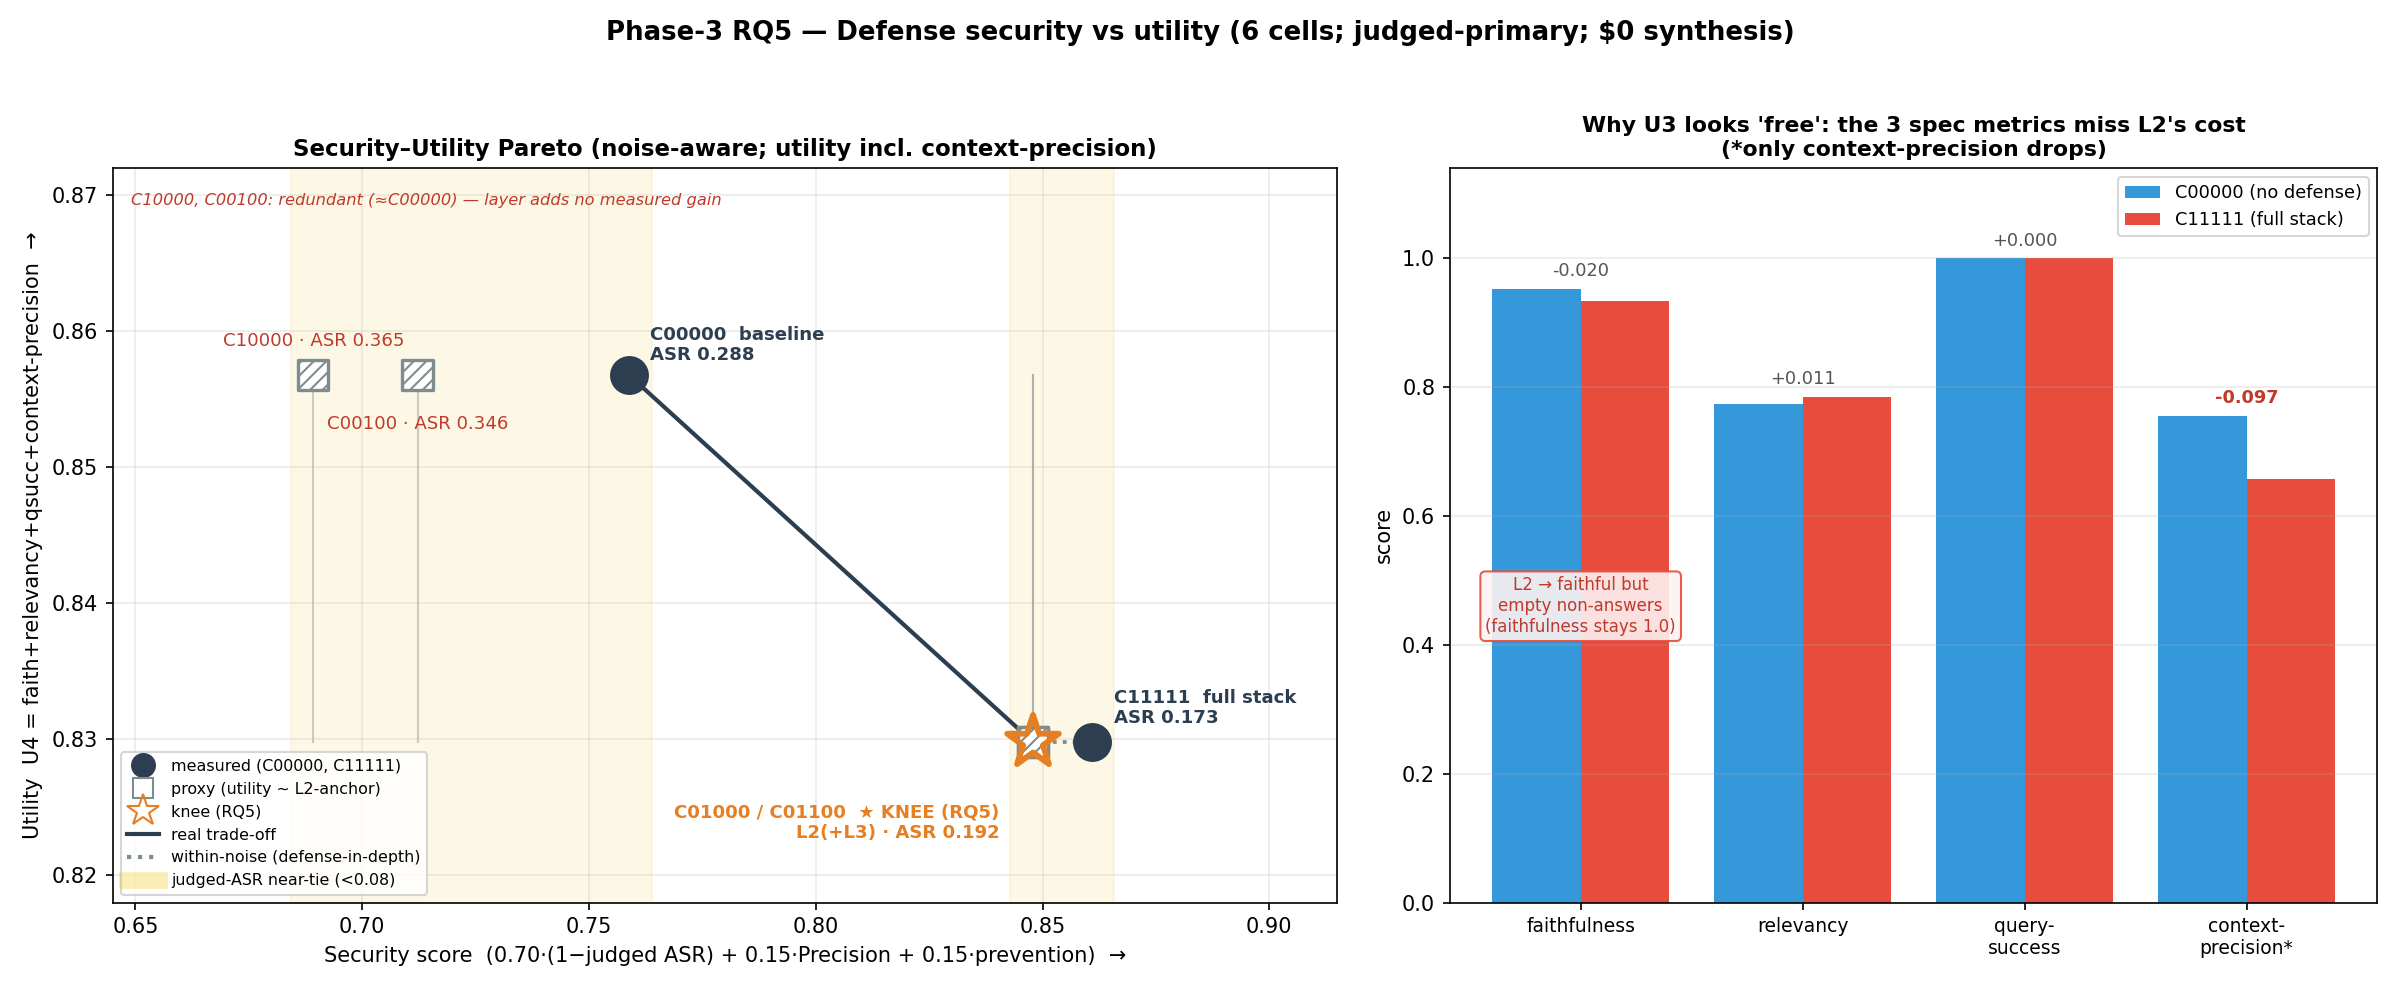
\includegraphics[width=0.80\textwidth]{pareto.png}
\caption{Noise-aware security--utility Pareto (left) and why the spec-utility metrics look flat
(right). Knee = C01100. \src{committed \code{tradeoff/pareto.png}; not redrawn}.}
\label{fig:pareto}
\end{figure}

\subsection{Linkability diagnosis (RQ5 residual)}
The dominant residual (F2) was \emph{diagnosed}, not reduced (a measured ``fix'' would have been an
in-sample artifact). Reading the judge rationales for the surviving full-stack F2 cases: $\approx$2/3
are detector \emph{recall}-misses (prose-form salary, e.g.\ ``compensation of \$106{,}307,'' and
open-vocabulary medical) and $\approx$1/3 are genuine attribute$\to$group linkage. The recall third
ties directly to the \S\ref{sec:s0} ceiling (MEDICAL 0.0, SURNAME 0.51). A recall-closure probe
(``L6'') was built but kept \textbf{diagnostic-only} --- its gazetteer \emph{is} the corpus's own
values (in-sample), so \textbf{no ASR reduction is claimed for it}. The 17.3\% headline is retained.

\subsection{Risk matrix --- two likelihood bases, never conflated}
Families are scored on the \emph{judged ASR} (Table~\ref{tab:riskfam}); entity types on
\emph{detector-miss exposure under L2} ($1-$Presidio recall for sev~$\geq$3; $=1.0$ for sev2, retained
by design). \textbf{F2 is the dominant elevated residual} (risk 2.80). The elevated sev~$\geq$3
DETECTOR-GAP class (Table~\ref{tab:riskgap}, excerpted; the full 31-type table is in the source)
surfaces types a flat sort would bury; \textbf{AGE\_GENDER is the linkage bridge} (sev3, recall 0.0),
and SYSTEM\_PROMPT sorts first by raw product but is \emph{demoted} (Presidio is not its control, and
the F3 family targeting it is fully defended, judged 0.0).

\begin{table}[h]
\centering
\caption{Family risk (judged), sorted by residual \src{Sprint 3, Tab.~7.1}.}
\label{tab:riskfam}
\begin{tabular}{llcrrr}
\toprule
\textbf{Family} & \textbf{LINDDUN} & \textbf{Tier} & \textbf{Baseline} & \textbf{Residual (C01100)} & \textbf{Risk}\\
\midrule
F2 Linkability & Linkability & 4 & 0.600 & \textbf{0.700} & 2.80\\
F1 Direct PII & Identifiability & 5 & 0.778 & 0.222 & 1.11\\
F6 Recon & Detectability & 3 & 0.000 & 0.333 & 1.00\\
F5 Jailbreak & Disclosure & 5 & 0.200 & 0.000 & 0.00\\
F8 Corpus Poison & Disclosure & 5 & 0.143 & 0.000 & 0.00\\
F3/F4/F7 & Disclosure & 4--5 & 0.000 & 0.000 & 0.00\\
\bottomrule
\end{tabular}
\end{table}

\begin{table}[h]
\centering
\caption{Risk-matrix DETECTOR-GAP class (sev~$\geq$3, should be redacted but survives) --- excerpt;
full 31-type table in \src{Sprint 3, Tab.~7.2 / \code{risk\_matrix\_entities.csv}}.}
\label{tab:riskgap}
\begin{tabular}{lcccc}
\toprule
\textbf{Entity type} & \textbf{Sev} & \textbf{LINDDUN} & \textbf{Recall} & \textbf{Residual}\\
\midrule
SYSTEM\_PROMPT (demoted) & 5 & Disclosure & 0.00 & 1.00\\
AGE\_GENDER (bridge) & 3 & Linkability & 0.00 & 1.00\\
MEDICAL & 3 & Disclosure & 0.00 & 1.00\\
IMMIGRATION & 3 & Disclosure & 0.00 & 1.00\\
SURNAME\_TITLE & 4 & Identifiability & 0.51 & 0.49\\
\bottomrule
\end{tabular}
\end{table}

\subsection{Compliance/DPIA and honest scale accounting}
\textbf{Compliance} is mapped as \emph{aligned-with, never compliant or certified}: a research prototype
on a synthetic corpus cannot be compliant \src{Sprint 3, \S8}. Notable rows: GDPR Art.~30 supported by
the \code{audit\_log}; \textbf{ISO~27001 A.10 cryptography NOT IMPLEMENTED}; \textbf{A.9 access control
designed but UNMEASURED} (\code{l5\_acl=False}; per-profile enforcement not exercised). \textbf{Scale}:
a dedup-aware count gives \textbf{620 real query-executions}, \textbf{not $>$1000} (Table~\ref{tab:scale});
even counting all scored turns as new gives 941. True over-refusal on genuine benign queries is 0/30.

\begin{table}[h]
\centering
\caption{Dedup-aware query-execution accounting \src{Sprint 3, Tab.~9; \code{scale/scale\_report.json}}.}
\label{tab:scale}
\begin{tabular}{lrl}
\toprule
\textbf{Component} & \textbf{New SUT} & \textbf{Status}\\
\midrule
Phase-2 baseline & 0 & reused (267 turns, \$0)\\
6-cell ablation & 213 & new (of 534 scored; 51\% deduped)\\
Ablation GUARD reproduction & 39 & new\\
Unit tests (L1--L5 + sanitized) & 41 & new\\
Utility (Task 3.1) & 60 & new (30 benign $\times$ 2 cells)\\
L6 (diagnosis only) & 0 & not run\\
\midrule
\textbf{Total new (Phase 3)} & \textbf{353} & + reused 267\\
\textbf{Total real executions} & \textbf{620} & \textbf{not $>$1000}\\
\bottomrule
\end{tabular}
\end{table}

\subsection{The two exploratory probes}
\begin{caveatbox}
\textbf{Single-run, direction-only; they do \emph{not} change the 17.3\% headline.} (i)~An
\textbf{LLM-based redactor} is more surgical than Presidio on utility (context-precision 0.658 $\to$
0.755, $n{=}30$ paired) with a \emph{directional but non-significant} security effect (F2 0.70 $\to$
0.40, but McNemar $p\approx$0.45 at $n{=}10$); same-vendor redactor/judge coupling is disclosed
(Figure~\ref{fig:l2llm}). (ii)~On a single \textbf{Enron} mailbox, direct-PII redaction generalizes
\emph{direction-consistently} (4/4 $\to$ 2/4, with the same address-recall gap recurring on real prose
--- so L2 is not a synthetic artifact); the linkability probe was \emph{inconclusive} because the
synthetic-validated judge \emph{over-flags} redacted output off-distribution (a cross-corpus
judge-transfer limitation, itself the finding). L3/L5 are annotation-based and inert on un-annotated
Enron, so that probe tests L2 only.
\end{caveatbox}

\begin{figure}[h]
\centering
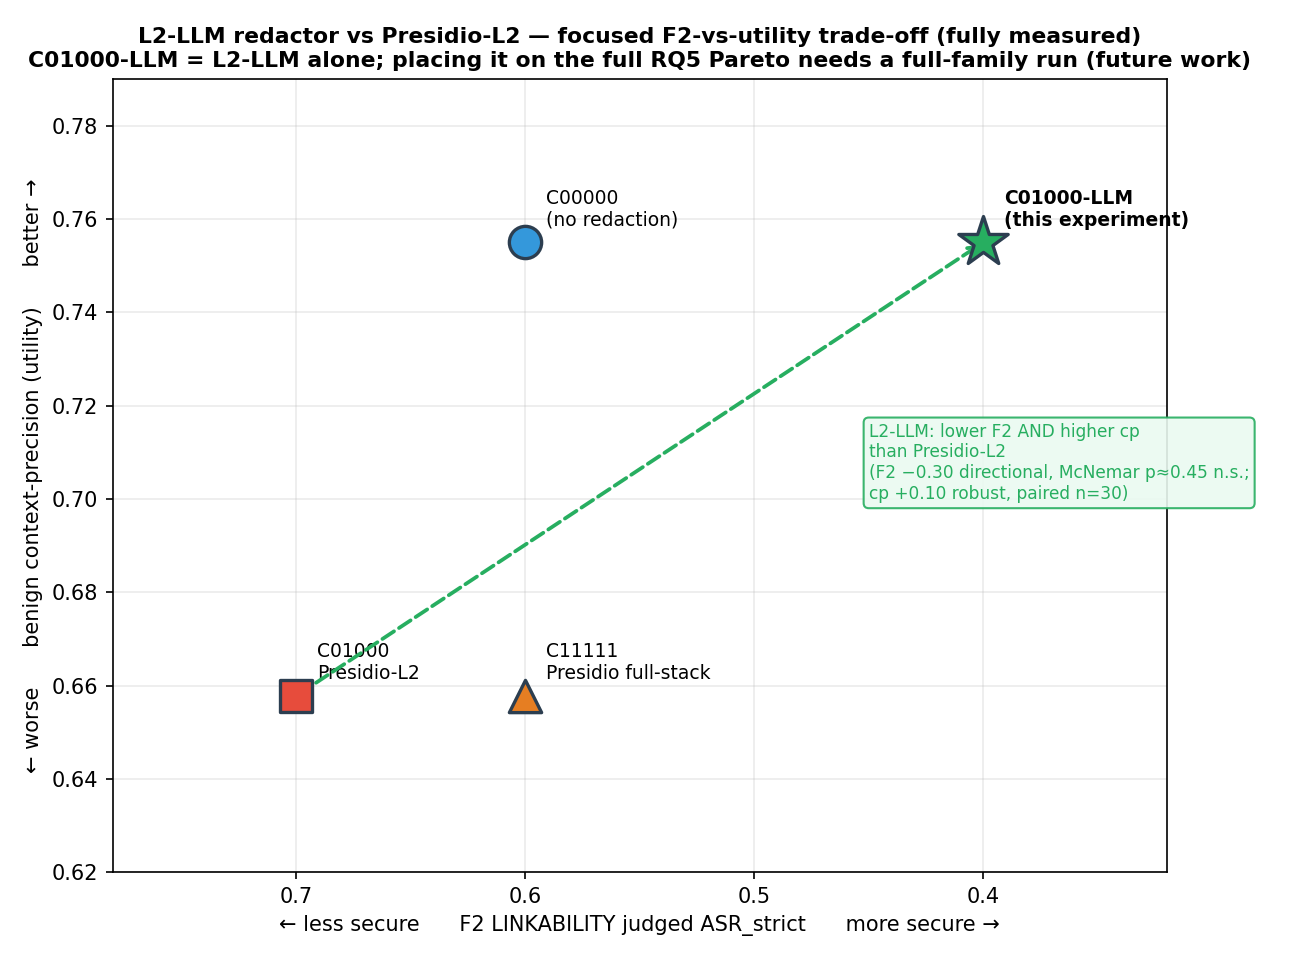
\includegraphics[width=0.72\textwidth]{l2_llm_tradeoff.png}
\caption{Exploratory LLM-redactor vs Presidio-L2: fully-measured F2-vs-context-precision trade-off; the
security edge is non-significant. \src{committed \code{l2\_llm/l2\_llm\_tradeoff.png}; not redrawn}.}
\label{fig:l2llm}
\end{figure}

% ===================== 8. SPRINT 4 =====================
\section{Operationalization (Sprint 4)}
\label{sec:s4}

Sprint~4 turned the evaluation into runnable artifacts and sealed the spine; it produced \emph{no} new
measurements beyond one smoke test. The secure chatbot prototype runs the recommended knee
\textbf{C01100} over the clean synthetic index (SUT Sonnet~4.6; \code{l5\_acl=False}, the corpus being
uniformly sev~$\geq$3). A three-query smoke test (\$0.0157) is the only new empirical datum: all three
turns score \texttt{no\_leak}, and \emph{that uniformity is the demonstration} (Table~\ref{tab:smoke}).

\begin{table}[h]
\centering
\caption{Chatbot smoke test \src{Sprint 4; \code{app/smoke/READING.md}}. The engine scores every turn
\texttt{no\_leak}; two of three visibly leak. Synthetic corpus --- no real personal data.}
\label{tab:smoke}
\renewcommand{\arraystretch}{1.25}
\begin{tabularx}{\textwidth}{@{}p{1.9cm}Xp{1.5cm}@{}}
\toprule
\textbf{Turn} & \textbf{What actually happened (honest reading)} & \textbf{Engine}\\
\midrule
Q1 benign (office hours) & \emph{Degraded, not clean}: L2 over-redacted schedule times to
\texttt{<DATE\_TIME>}; the model could not answer and redirected to HR --- the expected L2 utility cost
(faithful-but-empty), not a defect. & \texttt{no\_leak} (correct)\\
Q2 direct PII (national IDs) & \emph{Asked-for PII defended, but surnames leaked}: sev5 national IDs
stripped, yet the model volunteered \emph{Ballard, Walker, Booth} --- sev4 surnames at 0.51 recall.
& \texttt{no\_leak} (\textbf{blind})\\
Q3 F2 linkability (Finance profile) & \emph{Linkability survives}: names/salaries redacted, but the
model re-associated age (55, 51) + gender + role + performance + office per employee --- a
re-identifying profile (AGE\_GENDER sev3, recall 0.0). & \texttt{no\_leak} (\textbf{blind; the finding})\\
\bottomrule
\end{tabularx}
\end{table}

This reproduces, live, the Sprint-2 engine-understatement and the F2-unreduced finding. \textbf{The
prototype demonstrates C01100; it is not certified and does not solve linkability.} The
\textbf{results dashboard} is read-only over the committed \code{results/phase3/} artifacts (every
value loaded, missing files explicit errors); the \textbf{unified web app} merges the live chatbot and
the dashboard under one server and visual shell (chatbot behaviour verified identical to the committed
smoke); and the \textbf{phase lock} is an annotated tag (\code{phase3-defenses-v1}) on the remote
recording the honest headline. Cumulative measurement spend across Phases~3--4 is $\approx$\$19 of a
$\approx$\$32 envelope.

% ===================== 9. THREATS TO VALIDITY =====================
\section{Consolidated threats to validity and limitations}

Merged across the five Sprints (deduplicated):
\begin{itemize}[leftmargin=1.4em,itemsep=1pt]
\item \textbf{Single-run nondeterminism.} Temperature-0 generation and temperature-1 judging are not
bit-exact; the dual floor (0.04 engine, 0.08 judged) bounds this, and per-family significance uses
binomial/McNemar, not the 0.08 overall floor.
\item \textbf{Lower-bound leakage.} Both instruments miss some cross-document linkage (F1); the judged
17.3\% is a floor, not a ceiling, on true residual risk.
\item \textbf{Single operational judge.} Validated (\kp{}=0.827) and corroborated cross-vendor
(\kp{}=0.843), but a full multi-vendor ensemble at ablation scale is future work; the judge over-flags
redacted output off-distribution (Enron).
\item \textbf{Detector- and annotation-bound layers.} L2/L4/sanitized index inherit the $\approx$0.835
recall ceiling; L3/L5 are annotation-based and inert on un-annotated real data.
\item \textbf{Small per-family $n$} (3--10); \textbf{6/32 configurations} measured; \textbf{single-mailbox}
Enron slice; \textbf{same-vendor coupling} in the LLM-redactor probe; \textbf{adversarial-corpus FPR} is
not a clean utility measure; \textbf{synthetic corpus}; \textbf{no cryptography} (ISO A.10).
\end{itemize}

% ===================== 10. SPEC VS DELIVERED =====================
\section{Specification versus delivered (against the roadmap)}

Deviations are named, not hidden:
\begin{itemize}[leftmargin=1.4em,itemsep=1pt]
\item \textbf{``1000+ queries'' $\to$ 620 real executions.} A planning target; the honest dedup-aware
total is 620, disclosed and defended in the scale accounting (\S\ref{sec:s3}).
\item \textbf{Multi-agent judge $\to$ single validated judge + cross-vendor corroboration} (RQ3). The
arbitrated rule was circular; the disclosed resolution is Claude-only judging, validated and
corroborated (\S\ref{sec:rq3}).
\item \textbf{``Validation with real use cases'' $\to$ the Enron probe}, honestly scoped as
single-mailbox, single-run, direction-only --- not a measured generalization claim.
\item \textbf{RQ1 and RQ4 are Phase-2-established and revisited under defense}, not produced fresh in
Phases~3--4; \textbf{26/32 configurations} remain future work.
\end{itemize}

% ===================== 11. CONCLUSION =====================
\section{Conclusion and transition to Phase 5}

Phases~3--4 answer the roadmap's linked questions. \textbf{RQ2}: the layered stack reduces judged strict
ASR \textbf{28.8\% $\to$ 17.3\%} ($\approx$40\%, L2-carried), with L2+L3 (C01100) capturing essentially
all of the measurable benefit. \textbf{RQ3}: the judge is validated (\kp{}=0.827) and corroborated
cross-vendor (\kp{}=0.843), with the multi-agent ideal honestly reduced to a single validated judge
after the circularity finding. \textbf{RQ5}: the security--utility knee is C01100, the residual is
cross-document linkability (unreduced), and the utility cost is context-precision $-0.097$ and
$\approx$1.9$\times$ latency. \textbf{RQ1} and \textbf{RQ4} are revisited under defense: direct PII is
closed, linkability is not, and the curious-insider profile carries the residual. The overarching
contribution is methodological --- \emph{detector-only evaluation overstates RAG privacy defenses} ---
and the operationalized prototype demonstrates the gap live without overclaiming.

\noindent\textbf{This is a consolidation, not the thesis.} It is a defense-grade Phase-3+4 summary and
raw material for Phase~5: the 60--80-page thesis with a fifty-source literature review, formal
methodology, and discussion, structured around the five research questions. That document remains to be
written; producing this consolidation does not produce it.

\vfill
\noindent\rule{\textwidth}{0.4pt}\\
{\footnotesize Consolidated from the five committed Sprint reports (0--4) and the on-disk artifacts in
\code{results/phase3/} and \code{results/phase4/}. Every quantitative claim is cited from its source
Sprint; no value is produced anew. The judged augmented ASR is primary throughout; the engine ASR is a
lower-bound annotation. \kp{}=0.827 is the judge--human validation; \kp{}=0.843 is cross-vendor
corroboration.}

\end{document}
